\subsection[Mechanizm działania (Jakub Wyka)]{Mechanizm działania}
Na rysunku  ~\ref{fig:ethmechanizm} zostało przedstawiona infrastruktura potrzebna aby możliwe było skonfigurowanie urządzenia jako kartę sieciową. Jest to urządzenie wykonujące, podłączone do lokalnej sieci bezprzewodowej oraz do testowanego komputera za pomocą kabla USB.
Po odpowiedniej konfiguracji urządzenia wykonującego, testowany komputer automatycznie połączy się z nową siecią. Będzie ono widoczne jako połączenie Ethernet. W praktyce dostęp do internetu zapewniany będzie po kablu USB pomiędzy testowanym komputerem a urządzeniem testującym, które będzie pełniło funkcję karty sieciowej.
\begin{figure}[H]
    \centering
    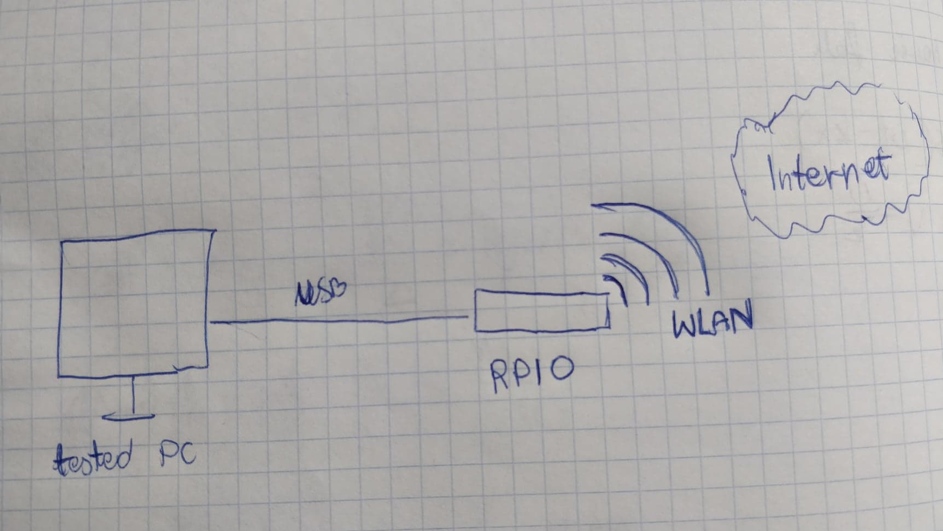
\includegraphics[width=\textwidth]{jw01}
    \caption{Schemat infrastruktury dla konfiguracji karty sieciowej}
    \label{fig:ethmechanizm}
\end{figure}